\section[EPA]{Einzelpartikelanalyse} % (fold)
\label{sec:einzelpartikelanalyse}
\subsection*{subsection name} % (fold)
\label{sub:subsection_name}

% subsection subsection_name (end)
\begin{frame}
	\frametitle{Einzelpartikelanalyse}
	\begin{figure}
		\includegraphics[width = 7cm]{pic/epa2.png}
	\end{figure}
	\begin{figure}
		\includegraphics[width = 8cm]{pic/epa_all.png}
	\end{figure}
\end{frame}

\begin{frame}
	\frametitle{Einzelpartikelanalyse}
	\begin{block}{Auswahl und Klassifizierung}
		\begin{itemize}
			\item Manuelle Auswahl der Partikel
			\item Gleiche Ausrichtung aller Partikel
			\item Klassifizierung
		\end{itemize}
	\end{block}
	\centering
	\begin{minipage}{3.5cm}
		\begin{figure}
			\includegraphics[width = 3.5cm]{pic/k_c_1.png}
		\end{figure}
	\end{minipage}
	\begin{minipage}{3.5cm}
		\begin{figure}
			\includegraphics[width = 3.5cm]{pic/k_c_2.png}
		\end{figure}
	\end{minipage}
	\begin{minipage}{3.5cm}
		\begin{figure}
			\includegraphics[width = 3.5cm]{pic/k_c_3.png}
		\end{figure}
	\end{minipage}
\end{frame}

\begin{frame}
	\frametitle{Einzelpartikelanalyse}
	\begin{block}{Erste Rekonstruktion}
		\begin{itemize}
			\item Klassensummen als Projektionen
			\item Startmodell aus Gaußschem Rauschen
			\item Kreuzkorrelation
		\end{itemize}
	\end{block}
	\begin{figure}
		\includegraphics[width = 5.5cm]{pic/recons.png}
	\end{figure}
\end{frame}

\begin{frame}
	\frametitle{Einzelpartikelanalyse}
	\begin{block}{3D Refinement}
		\begin{itemize}
			\item Simulation von 2D Projektionen
			\item Vergleich und Ausrichtung der Partikel
			\item Radon Transformation
		\end{itemize}
	\end{block}
	\begin{figure}
		\includegraphics[width = 8cm]{pic/epa1.png}
	\end{figure}
\end{frame}

\begin{frame}
	\frametitle{Einzelpartikelanalyse}
	\begin{figure}
		\includegraphics[width = 11cm]{pic/radon.jpg}
		\hspace{3cm}
	\end{figure}
	\vspace{3cm}
\end{frame}

\begin{frame}
	\frametitle{Einzelpartikelanalyse}
	\begin{figure}
		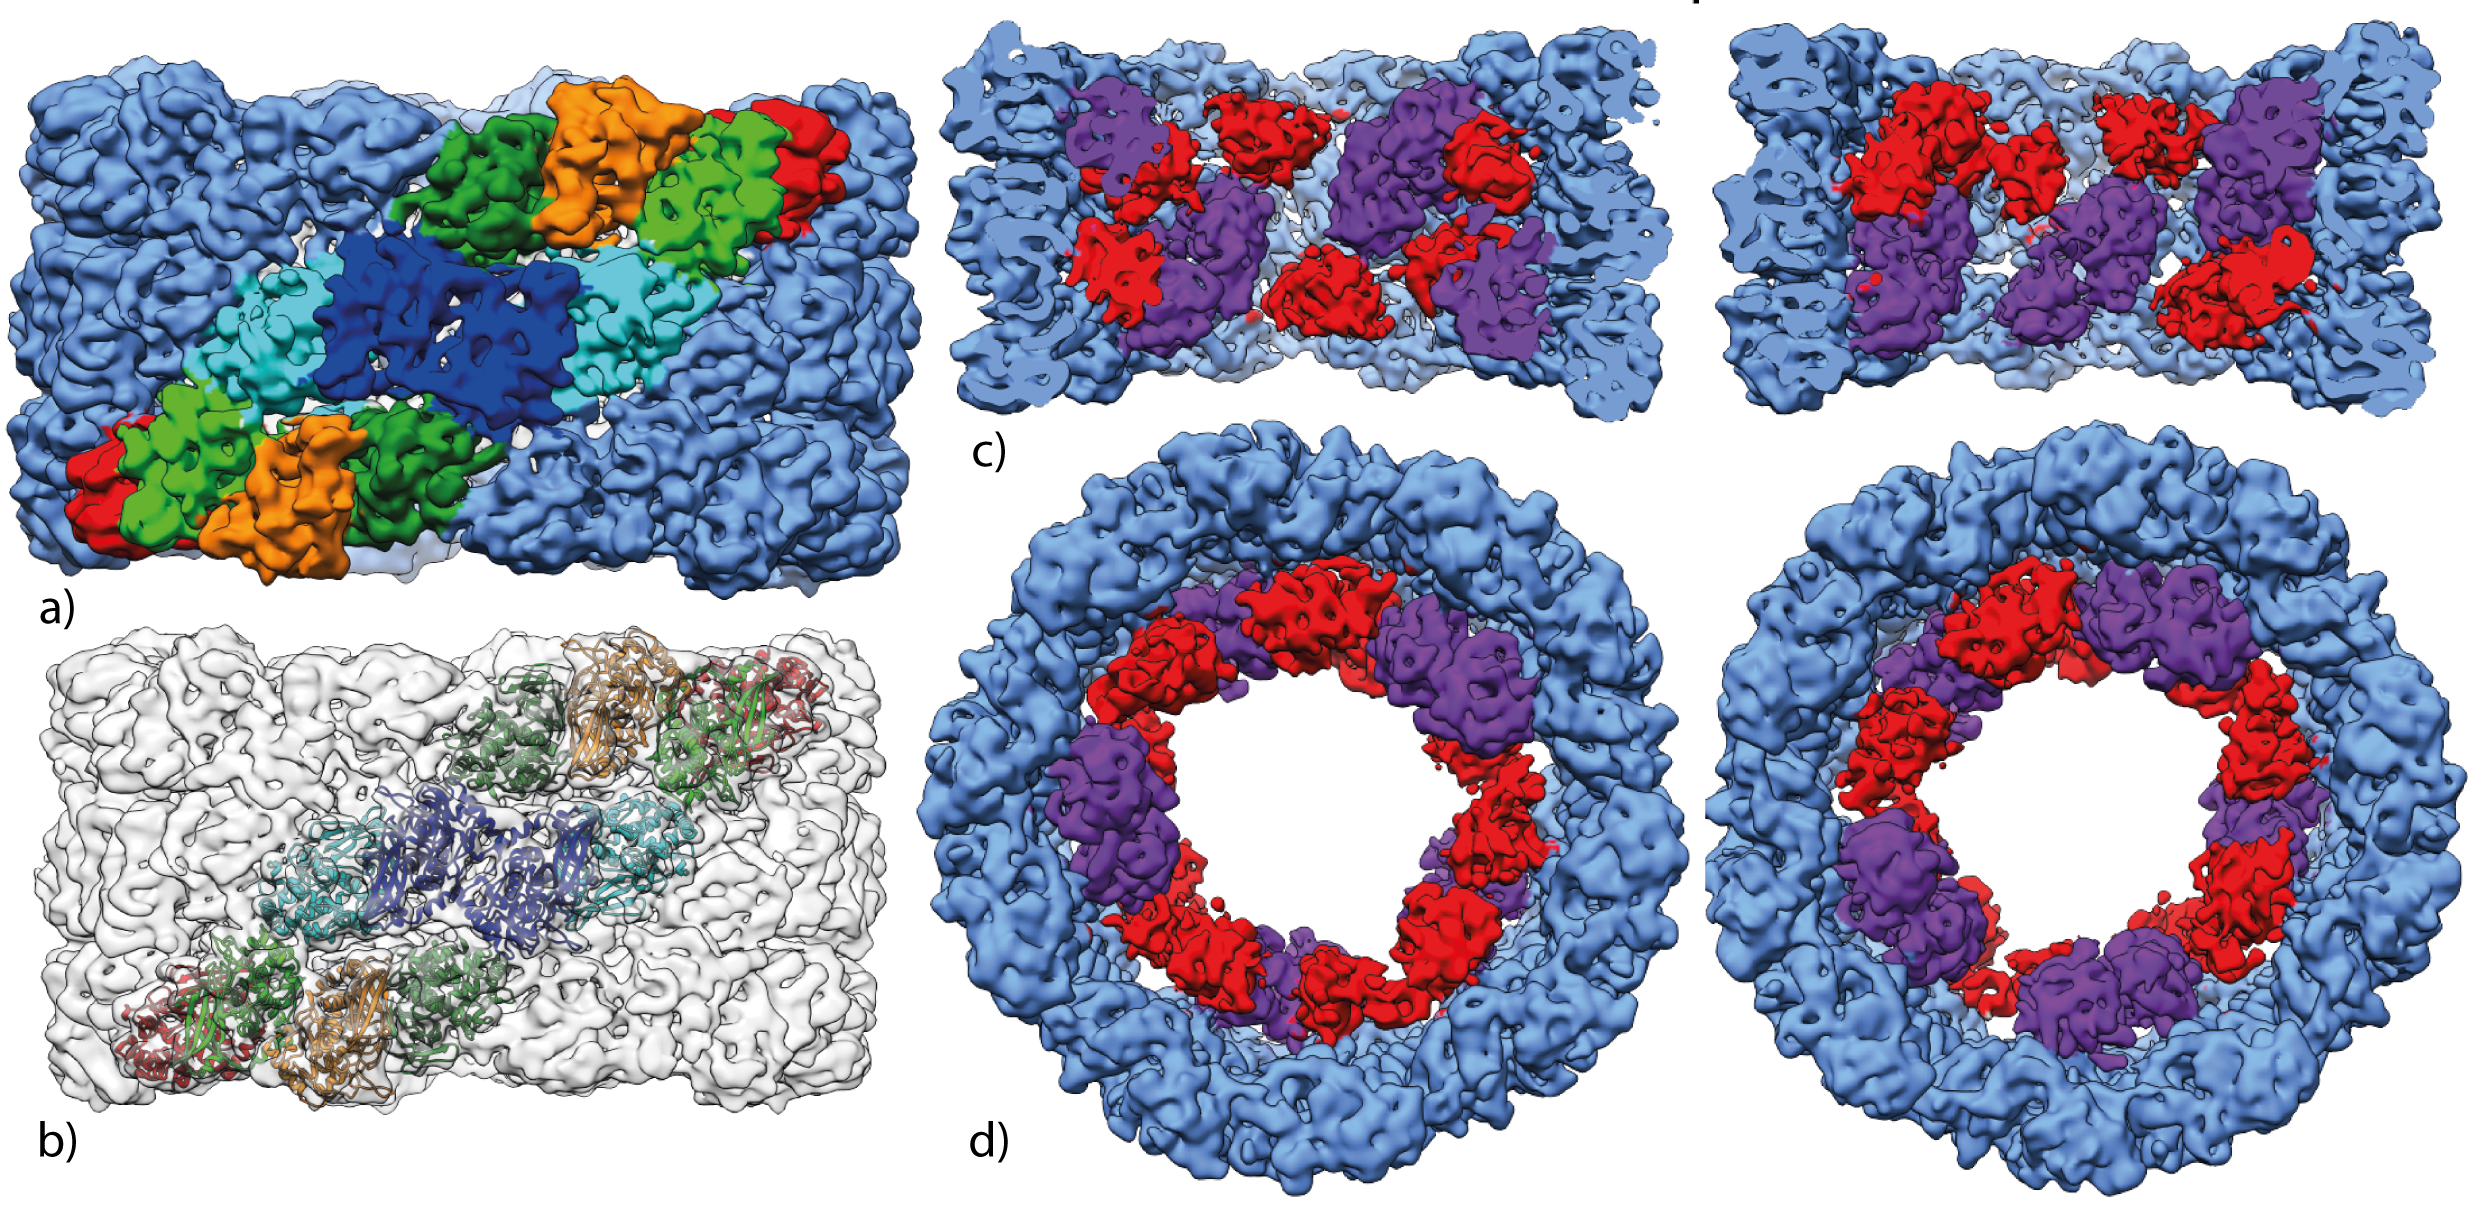
\includegraphics[width = 11cm]{pic/diezwei.png}
	\end{figure}
\end{frame}